% Q6：线型按原页复现。空间位置仅作示意，不按比例。
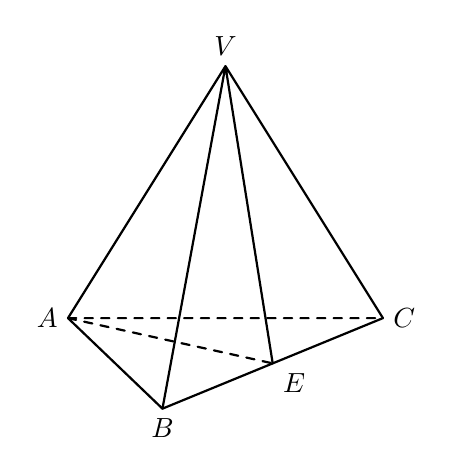
\begin{tikzpicture}[line cap=round,line join=round,thick]
  \coordinate (V) at (0,3.2);
  \coordinate (A) at (-2.0,0);
  \coordinate (B) at (-0.8,-1.15);
  \coordinate (C) at (2.0,0);
  \coordinate (E) at (0.6,-0.575);

  % Visible pyramid edges and the median in face VBC.
  \draw (V)--(A) (V)--(B) (V)--(C) (V)--(E);
  \draw (A)--(B)--(C);

  % Hidden rear base edge and the indicated segment AE.
  \draw[dashed] (A)--(C) (A)--(E);

  \node[above] at (V) {$V$};
  \node[left] at (A) {$A$};
  \node[below] at (B) {$B$};
  \node[right] at (C) {$C$};
  \node[below right] at (E) {$E$};
\end{tikzpicture}
